\section{Delayed release and the low-energy excess}\label{sec:19.6}

A close Frenkel pair in silicon holds 6.8 to \SI{7.5}{eV} (\cref{sec:7.4}), and at \SI{10}{mK} it can give them back only by tunneling. For an estimated barrier of \SI{0.1}{eV} over \SI{1.5}{\angstrom} the two-parabola tunneling exponent is 27.5, about \SI{14}{\percent} above the largest exponent that allows recombination within a year (\cref{sec:16.8-hop}). Whether the pair releases its energy during a run or keeps it for good thus depends on one number that is not known. Meanwhile cryogenic detectors with thresholds of tens of eV record an excess of events that rises toward threshold and decays over days after cooldown. A silicon crystal glued to its holder shows more than a hundred times the rate of an identical crystal hung from wire bonds~\cite{anthonypetersen2024stress}. Energy stored in defects is the obvious suspect. Its release at millikelvin obeys an exact sum rule, which fixes how much energy delayed events can carry and at what energy per event; together with energy conservation it bounds the excess, and it leaves collective release of elastic energy as the candidate.

\subsection{Defect kinetics at millikelvin}\label{sec:19.6-kinetics}

At $t_{\mathrm{pr}}$ the recoil leaves the crystal in one of a set of configurations $i$, each a basin of $E^{\mathrm{ad}}$ with the configurational energy $E^{\mathrm{conf}}_i$, the minimum of the basin measured from the minimum of the perfect crystal (\cref{eq:19.1-partition}). The perfect crystal is one of them, with $E^{\mathrm{conf}} = 0$. Let $p_i(t)$ be the probability that the defect complex is in configuration $i$ at time $t$, and $\varGamma_{ij}$ the rate of a hop from $i$ to $j$. Hops are rare compared with the vibrations inside a basin, so the populations obey the master equation
\begin{equation}
  \frac{\dd p_i}{\dd t} = \sum_{j\ne i}\bigl[\varGamma_{ji}\,p_j - \varGamma_{ij}\,p_i\bigr] ,
  \qquad p_i(t_{\mathrm{pr}}) \text{ from the partition at } t_{\mathrm{pr}} .
  \label{eq:19.6-master}
\end{equation}
The stored energy at time $t$ is the mean configurational energy, $E_{\mathrm{st}}(t) = \sum_ip_i(t)E^{\mathrm{conf}}_i$, which equals the $E_{\mathrm{st}}$ of the partition at $t = t_{\mathrm{pr}}$.

The rates at millikelvin are tunneling rates. A barrier of chemical size cannot be crossed thermally, and below the crossover temperature $T_\times$ of \cref{eq:16.8-Tx}, tens of kelvin for an atom, every hop goes through the barrier (\cref{sec:16.8-hop}). A hop from $i$ to $j$ releases $\varepsilon^{\mathrm{hop}}_{ij} = E^{\mathrm{conf}}_i - E^{\mathrm{conf}}_j$, and its tunneling amplitude is $\Delta_0 = \omega_{\mathrm{w}}\ee^{-\lambda_{\mathrm{tun}}}$ in the notation of \cref{sec:16.7}. The golden rule \cref{eq:C.20-rate} gives the rate as $\Delta_0^2/4$ times the time integral of the bath correlation at the energy released. Let $A(\varepsilon)$ be the line shape, the probability per unit energy that the bath accepts the energy $\varepsilon$. Then
\begin{equation}
  \varGamma_{ij} = \frac{\pi}{2}\,\omega_{\mathrm{w}}^2\,\ee^{-2\lambda_{\mathrm{tun}}}\,A\bigl(\varepsilon^{\mathrm{hop}}_{ij} + \Delta E_{\mathrm{zp},ij}\bigr) ,
  \label{eq:19.6-hop}
\end{equation}
where $\Delta E_{\mathrm{zp},ij}$ is the decrease of the zero-point energy of the local modes in the hop, so that the argument is the energy the bath actually receives. For the two-level systems of \cref{sec:16.8} the energy is below the top of the phonon band and one phonon takes it; then $A(\varepsilon) = J_{\mathrm{s}}(\varepsilon)\coth(\varepsilon/2T)/\pi\varepsilon^2$, which turns \cref{eq:19.6-hop} into \cref{eq:16.8-golden}. An eV release is far above the phonon band, so the bath can take it only as many quanta at once, in the local modes $k$ that are displaced between the two minima, with Huang--Rhys factors $S_{\mathrm{HR},k}$ and the reorganization energy $E_{\mathrm{reorg}} = \sum_kS_{\mathrm{HR},k}\omega_k$ of \cref{eq:E.22-SHR}. At $T \ll \omega_k$ the correlation of one displaced mode is the Poisson series of \cref{eq:5.6-poisson}, and the size of the rearrangement decides between two regimes.

If the hop is a small rearrangement, $E_{\mathrm{reorg}} \ll \varepsilon^{\mathrm{hop}}$, the energy must go into $n_q = \varepsilon/\omega_{\mathrm{acc}}$ quanta of modes that are barely displaced. For one accepting mode of energy $\omega_{\mathrm{acc}}$ and total factor $S$, the Poisson weight of $n_q$ quanta gives $A(\varepsilon)\,\omega_{\mathrm{acc}} = \ee^{-S}S^{n_q}/n_q!$, the energy-gap law. For $S = 1$, $\omega_{\mathrm{acc}} = \SI{60}{meV}$ and $\varepsilon = \SI{1}{eV}$ it is $2.7\times10^{-15}$, which adds 16.8 to the tunneling exponent. If instead the hop is a large rearrangement, $E_{\mathrm{reorg}} \approx \varepsilon^{\mathrm{hop}}$, the reaction coordinate itself takes the energy. Then $A$ is a Gaussian of width $(\sum_kS_{\mathrm{HR},k}\omega_k^2)^{1/2}$ centered at $E_{\mathrm{reorg}}$, and there is no gap suppression. The two-state reduction behind \cref{eq:19.6-hop} is then not controlled either, and the rate is the instanton rate on the full surface (\cref{sec:16.8-hop}). Taking the prefactor, of order $\omega_{\mathrm{w}}$, as $\varGamma_0 = \SI{e13}{s^{-1}}$, a hop happens within the observation time $t_{\mathrm{obs}}$ if
\begin{equation}
  2\lambda_{\mathrm{tun}} + \ln\frac{1}{\omega_{\mathrm{w}}A(\varepsilon)} \le \ln\bigl(\varGamma_0t_{\mathrm{obs}}\bigr) ,
  \label{eq:19.6-window}
\end{equation}
and for one year the right side is 47.2. With $\omega_{\mathrm{w}}A \approx 1$ this is the bound $\lambda_{\mathrm{tun}} \le 23.6$ of \cref{sec:16.8-hop}. With the energy-gap factor above it becomes $\lambda_{\mathrm{tun}} \le 6.8$, and for a \SI{7}{eV} release the logarithm of the factor is about 440, so a weakly coupled eV release never happens.

For a close Frenkel pair in silicon the two-parabola exponent $\lambda_{\mathrm{tun}} = (d_{\mathrm{tun}}/2)(2M_\kappa V_{\mathrm{b}})^{1/2}$ with $M_\kappa = \SI{26.16}{GeV}$, $V_{\mathrm{b}} = \SI{0.1}{eV}$ and $d_{\mathrm{tun}} = \SI{1.5}{\angstrom}$ is 27.5, and a quartic barrier of the same height and width raises it by $4/3$, to 36.7. In the weak-coupling regime the pair is frozen. In the strong-coupling regime it recombines within a year only if the true exponent lies at least \SI{14}{\percent} below the two-parabola value. A split interstitial in aluminum, with an estimated barrier of \SI{0.1}{eV} over \SI{1.4}{\angstrom}, has 25.2 and needs \SI{6}{\percent}. Aluminum is superconducting at these temperatures, so its conduction electrons do not take the energy (\cref{sec:16.8-electron}). Whether either defect releases its energy therefore depends on one calculation per path (\cref{sec:19.6-open}).

\subsection{The release-path sum rule}\label{sec:19.6-sumrule}

Every hop puts energy into the crystal, and a detector sees its distribution in energy and time. For one seed, the expected number of hops per unit time and per unit released energy is
\begin{equation}
  \mathcal{R}_{\mathrm{hop}}(E, t) = \sum_{i\ne j}p_i(t)\,\varGamma_{ij}\,\delta\bigl(E - \varepsilon^{\mathrm{hop}}_{ij}\bigr) ,
  \label{eq:19.6-Rhop}
\end{equation}
with the configurational energy in the delta function. Its integral over $E$ and $t$ is the expected number of hops $\langle N_{\mathrm{hop}}\rangle$, not one: a pair may pass through several configurations before it recombines. The energy it releases is fixed by its end points alone.
\begin{keyresult}[Release-path sum rule]
For populations that obey \cref{eq:19.6-master} on a closed set of configurations,
\begin{equation}
  \int_{t_{\mathrm{pr}}}^{t}\dd t'\int\dd E\;E\,\mathcal{R}_{\mathrm{hop}}(E, t') = E_{\mathrm{st}} - E_{\mathrm{st}}(t) ,
  \label{eq:19.6-sumrule}
\end{equation}
the stored energy of the partition minus the energy still stored at $t$.
\end{keyresult}
\noindent By \cref{eq:19.6-master},
\begin{equation*}
  \frac{\dd}{\dd t}\sum_ip_iE^{\mathrm{conf}}_i = \sum_{i\ne j}\bigl(\varGamma_{ji}p_j - \varGamma_{ij}p_i\bigr)E^{\mathrm{conf}}_i
  = -\sum_{i\ne j}\varGamma_{ij}\,p_i\bigl(E^{\mathrm{conf}}_i - E^{\mathrm{conf}}_j\bigr) = -\int\dd E\;E\,\mathcal{R}_{\mathrm{hop}}(E, t) ,
\end{equation*}
where the middle step exchanges the labels in the first term. Integrating from $t_{\mathrm{pr}}$ to $t$ gives \cref{eq:19.6-sumrule}. Neither detailed balance nor any model of the rates enters, so the rule holds for every rate law of \cref{sec:19.6-kinetics} and also for rates that change in time. These include the rates stimulated by a heat pulse, by illumination or by the carriers of a later event.

The rule is exact under five conditions on how a calculation accounts for the energy: every hop counted, one table of configurational energies, photons counted as escaped energy, no probability leaving the listed configurations, and configurational energies throughout. Every hop must be counted, including uphill hops with $\varepsilon^{\mathrm{hop}} < 0$, in which the defect absorbs heat from the lattice. The partition and the release paths must use one table of configurational energies, from one potential and one cell, as \cref{sec:19.1-md} requires; otherwise the two sides differ by the error of the potential, a few tenths of an eV. A hop that emits a photon still releases its energy, which then appears among the escaping quanta of the balance law of \cref{sec:19.5} instead of the phonons. No probability may leave the listed configurations, $\sum_ip_i(t) = 1$: the master equation describes one seed, and recombination of an interstitial with the vacancy of another event lies outside it, since it needs the joint state of both. Finally, the energies are configurational. The energy that the bath receives in a hop is $\varepsilon^{\mathrm{hop}}_{ij} + \Delta E_{\mathrm{zp},ij}$, where the zero-point change is below a tenth of an eV, an estimate (\cref{sec:19.5-law}). The zero-point changes add up along any path to the zero-point change of the end basin, which \cref{sec:19.1-partition,sec:19.5-law} count in the phonons, not in $E_{\mathrm{st}}$. Read with these conditions, \cref{eq:19.6-sumrule} is the stored-energy term of the balance law \cref{eq:19.5-balance}: what leaves $E_{\mathrm{st}}(t)$ enters the phonons, at the energies and times of $\mathcal{R}_{\mathrm{hop}}$.

\begin{workedexample}{The release-path sum rule for one Frenkel pair}\label{we:19-sumrule}
Take a close Frenkel pair C in silicon with $E^{\mathrm{conf}}_{\mathrm{C}} = \SI{7.0}{eV}$, which can recombine directly to the perfect crystal 0 or first relax into a bond defect B with $E^{\mathrm{conf}}_{\mathrm{B}} = \SI{2.8}{eV}$, both inside the ranges of \cref{sec:7.4}. Separation to an isolated vacancy and interstitial, which costs 0.6 to \SI{2.9}{eV} more, is closed at \SI{10}{mK}. No path of this kind has been computed, so we take illustrative strong-coupling exponents in \cref{eq:19.6-window}, with $\varGamma = \varGamma_0\ee^{-2\lambda_{\mathrm{tun}}}$: $\lambda_{\mathrm{tun}} = 22.5$ for C$\to$B, 24.0 for C$\to$0 and 25.0 for B$\to$0. The rates are $\varGamma_{\mathrm{CB}} = 2.86\times10^{-7}$, $\varGamma_{\mathrm{C0}} = 1.43\times10^{-8}$ and $\varGamma_{\mathrm{B0}} = 1.93\times10^{-9}\,\si{s^{-1}}$. The pair leaves C after \SI{38.5}{days} on average, through B with probability $\varGamma_{\mathrm{CB}}/(\varGamma_{\mathrm{CB}} + \varGamma_{\mathrm{C0}}) = 0.953$.

The master equation for three states is solved by two exponentials, $p_{\mathrm{C}} = \ee^{-\varGamma_{\mathrm{C}}t}$ with $\varGamma_{\mathrm{C}} = \varGamma_{\mathrm{CB}} + \varGamma_{\mathrm{C0}}$, and $p_{\mathrm{B}} = \varGamma_{\mathrm{CB}}(\ee^{-\varGamma_{\mathrm{C}}t} - \ee^{-\varGamma_{\mathrm{B0}}t})/(\varGamma_{\mathrm{B0}} - \varGamma_{\mathrm{C}})$. After one year $p_{\mathrm{C}} = 10^{-4}$, $p_{\mathrm{B}} = 0.902$ and $p_0 = 0.098$, and the stored energy is $E_{\mathrm{st}}(t) = 0.902\times\SI{2.8}{eV} = \SI{2.526}{eV}$. The expected numbers of hops are $\varGamma_{ij}\int_0^t p_i\,\dd t'$: 0.9525 hops C$\to$B releasing \SI{4.2}{eV} each, 0.0474 hops C$\to$0 releasing \SI{7.0}{eV}, and 0.0505 hops B$\to$0 releasing \SI{2.8}{eV}. Together they release
\begin{equation*}
  0.9525\times\SI{4.2}{eV} + 0.0474\times\SI{7.0}{eV} + 0.0505\times\SI{2.8}{eV} = \SI{4.474}{eV} = \SI{7.0}{eV} - \SI{2.526}{eV} ,
\end{equation*}
as \cref{eq:19.6-sumrule} requires, in $\langle N_{\mathrm{hop}}\rangle = 1.05$ hops, \SI{4.26}{eV} per hop. After ten years \SI{5.539}{eV} has been released in 1.43 hops, and after a hundred years \SI{6.994}{eV} in 1.95 hops: the number of hops depends on the path, the energy only on the end points. A sensor that absorbs a quarter of the phonon energy of a release, as the sensors of the glued and suspended crystals do~\cite{anthonypetersen2024stress}, which absorb phonons before they thermalize, records the three kinds of hop as events of 1.05, 1.75 and \SI{0.70}{eV}, each shifted by a quarter of its zero-point change.
\end{workedexample}

\subsection{The delayed-release spectrum}\label{sec:19.6-spectrum}

A detector sees the sum of $\mathcal{R}_{\mathrm{hop}}$ over all seeds, from the recoils of earlier events and from the defects frozen in at cooldown, with each release converted into a recorded energy. A release of energy $\varepsilon$ puts $\varepsilon + \Delta E_{\mathrm{zp}}$ into athermal phonons, or into a photon on the radiative branch, and the sensor absorbs a fraction $f_{\mathrm{ph}}$ of the phonon energy, which depends on where the release happens and on the phonon spectrum. A release is an event only if $f_{\mathrm{ph}}(\varepsilon + \Delta E_{\mathrm{zp}}) \ge E_{\mathrm{th}}$. Below threshold it is heat, a load on the sensor that adds to its noise but makes no event.

Defects frozen in at cooldown follow the same kinetics, and two families dominate. The first family, the two-level systems of the amorphous films and glues near a detector, relaxes by emitting single phonons of energy $\Delta_{\mathrm{tl}}$ (\cref{sec:16.8}). After a quench from the freezing temperature $T_{\mathrm{frz}}$ to $T_{\mathrm{lo}}$, a defect of splitting $\Delta_{\mathrm{tl}}$ keeps the excess population $\frac12[\tanh(\Delta_{\mathrm{tl}}/2T_{\mathrm{lo}}) - \tanh(\Delta_{\mathrm{tl}}/2T_{\mathrm{frz}})]$, and the uniform density in $\lambda_{\mathrm{tun}}$ makes the fraction relaxing per unit time $1/2t$. The steps of \cref{eq:16.8-heat}, kept at fixed splitting, give the number of phonons emitted per unit energy and time by a volume $\Vol$,
\begin{equation}
  \frac{\dd\mathcal{R}_{\mathrm{TLS}}}{\dd E} = \frac{\bar P\Vol}{4t}\Bigl[\tanh\frac{E}{2T_{\mathrm{lo}}} - \tanh\frac{E}{2T_{\mathrm{frz}}}\Bigr] ,
  \label{eq:19.6-tls}
\end{equation}
whose first moment is \cref{eq:16.8-heat}. The mean quantum is $1.19\,T_{\mathrm{frz}}$, \SI{0.49}{meV} for $T_{\mathrm{frz}} = \SI{4.8}{K}$: the release of a glass is all heat, \SI{46}{pW} per gram of fused silica an hour after cooling (\cref{we:16-heat}), and none of it can be an event.

The second family is the point defects of the crystal itself, close Frenkel pairs and bond defects from earlier recoils, which release eV per hop in the strong-coupling regime and nothing in the weak one. \Cref{fig:19-release} shows both. Their time laws depend on the distribution of the paths. A uniform distribution of tunneling exponents leads to $1/t$, as for the glass, and a single path to an exponential. Correlated recombination of a pair that diffuses in three dimensions follows the first-passage tail $t^{-3/2}$. The time law alone, however, does not identify the source, since stress relaxation in a glue also leads to $1/t$ (\cref{sec:19.6-lee}).

\begin{figure}[tbp]
  \centering
  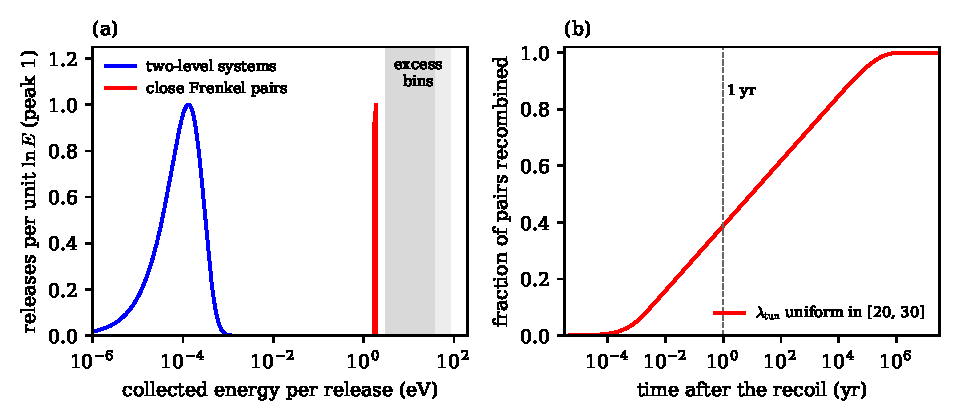
\includegraphics[width=\linewidth]{figures/ch19/fig19_5.pdf}
  \caption{Delayed releases from two defect families. (a) Distribution of the energy one release gives a sensor that absorbs a fraction $f_{\mathrm{ph}} = 0.25$ of the phonon energy, per unit logarithm of the energy, each family scaled to a peak of one. Blue: two-level systems frozen at $T_{\mathrm{frz}} = \SI{4.8}{K}$ and relaxing at \SI{10}{mK}, \cref{eq:19.6-tls}, mean quantum \SI{0.49}{meV}. Red: recombination of close Frenkel pairs in silicon, with configurational energies spread uniformly between 6.8 and \SI{7.5}{eV} (\cref{sec:7.4}), zero-point changes neglected. Gray: the 3--38 and 38--\SI{85}{eV} bins of energy absorbed in the sensor in which a glued silicon crystal shows its excess of events~\cite{anthonypetersen2024stress}. (b) Fraction of a family of close pairs recombined by time $t$, for strong coupling, $\varGamma = \SI{e13}{s^{-1}}\,\ee^{-2\lambda_{\mathrm{tun}}}$, with $\lambda_{\mathrm{tun}}$ spread uniformly between 20 and 30, an illustrative range around the two-parabola estimates. The fraction grows as $\ln t$ (a rate $\propto 1/t$) between \SI{6.5}{h} and $3.6\times10^5$ years; 0.39 of the pairs recombine within the first year. In the weak-coupling regime none does.}
  \label{fig:19-release}
\end{figure}

A close pair gives a sensor that absorbs a quarter of the phonons between 1.70 and \SI{1.88}{eV}, below the lowest bin of the excess (\cref{fig:19-release}(a)), and a two-level system gives a ten-thousandth of that. Single releases add to the heat load and, through the spectrum, to the noise of a sensor with a threshold of an eV or less; for thresholds of a few eV they are invisible. Amorphous pockets left by keV recoils are the one point-defect source that releases more at once: a pocket that recrystallizes releases of order \SI{0.1}{eV} per atom, an estimate, so a pocket of 120 atoms gives \SI{3}{eV} to such a sensor.

The inputs of these rates are computable from first principles. Barriers and minimum-energy paths come from the nudged elastic band, which relaxes a chain of configurations between the two minima onto the path, on the density-functional or machine-learned surface, the Huang--Rhys factors from the Hessians at both minima, and the exponent along the true path from ring-polymer instantons (\cref{app:E.22}). The sum rule \cref{eq:19.6-sumrule} is the acceptance test of the kinetic Monte Carlo, the stochastic sampling of hop sequences that turns the rates into $\mathcal{R}_{\mathrm{hop}}$.

\subsection{Defectons}\label{sec:19.6-defecton}

A light defect that tunnels between equivalent sites faster than the disorder around it can detune them becomes delocalized. This matters for a detector because a mobile defect reaches its partner, or a surface, on a time set by its band and not by a barrier. If the defect at site $\vect{r}$ tunnels to each neighbor with amplitude $A_{\mathrm{dfn}}$, the Bloch combinations of the localized states are stationary, and the defect becomes a quasiparticle, a defecton, with a band
\begin{equation}
  \varepsilon^{\mathrm{dfn}}(\vect{k}) = E^{\mathrm{loc}} - A_{\mathrm{dfn}}\sum_{i=x,y,z}\cos k_ia ,
  \label{eq:19.6-band}
\end{equation}
on a simple cubic lattice of spacing $a$~\cite[Eqs.~(1)--(3)]{pushkarov2004quantum}. The band width is $\Delta_{\mathrm{dfn}} = zA_{\mathrm{dfn}}$, with $z = 6$ neighbors, the mass at the bottom $1/A_{\mathrm{dfn}}a^2$, and the speed at most $A_{\mathrm{dfn}}a$. In solid helium, where defectons were first proposed, a ${}^3$He impurity has $\Delta_{\mathrm{dfn}} \sim \SI{e-4}{K}$; the light interstitials of metals, hydrogen in niobium for example, are candidates in the materials of detectors~\cite{pushkarov2004quantum}. In a hop the defecton cannot change its energy by more than $\Delta_{\mathrm{dfn}}$, so a gradient of the potential energy $\phi$ with $|\nabla\phi|a > \Delta_{\mathrm{dfn}}$ localizes it~\cite[Eq.~(17)]{pushkarov2004quantum}. Around a defect whose elastic interaction falls as $\phi = V_0(a/r)^3$, the gradient criterion reads $3V_0(a/r)^4 > \Delta_{\mathrm{dfn}}$, and the region $r < R_0 = a(3V_0/\Delta_{\mathrm{dfn}})^{1/4}$ is closed to band motion.

In a perfect crystal at $\Delta_{\mathrm{dfn}} \ll T$ the defecton moves through the band ballistically between collisions with phonons, and its diffusion constant falls as $T^{-9}$. The exponent follows from four facts: the kinematics of a narrow band, the Rayleigh form of two-phonon scattering, the small momentum change per collision, and the band velocity. First, the defecton cannot absorb or emit one phonon: that needs $|\varepsilon^{\mathrm{dfn}}(\vect{k} + \vect{Q}) - \varepsilon^{\mathrm{dfn}}(\vect{k})| = \bar cQ$, and the left side is at most $A_{\mathrm{dfn}}aQ$, far below $\bar cQ$ for a narrow band. The leading process is therefore two-phonon scattering, $\vect{Q} \to \vect{Q}'$ with $\omega' \simeq \omega$. Second, its amplitude is proportional to $\omega$. For a coupling quadratic in the strain, the elastic inhomogeneity of the defect, the amplitude carries $QQ'/(\omega\omega')^{1/2} \propto \omega$. The linear deformation coupling at second order has two time orderings with energy denominators $\pm\omega$ that cancel at leading order, and what remains is the second difference of the band, $\propto A_{\mathrm{dfn}}a^2QQ'$, again $\propto\omega$. The cross-section is therefore $\propto (Qa)^4$, Rayleigh scattering~\cite[Eq.~(49)]{pushkarov2004quantum}. Third, the number of thermal phonons grows as $T^3$, so the collision rate grows as $T^7$; but each collision changes the crystal momentum by at most about $T/\bar c$, much less than $1/a$~\cite[Eq.~(54)]{pushkarov2004quantum}, and $(1/Qa)^2 \propto T^{-2}$ collisions are needed to randomize it. The transport rate grows as $T^9$. Fourth, $D = v^2\tau_{\mathrm{tr}}/3$ with $v \sim A_{\mathrm{dfn}}a$ gives $D \propto \Delta_{\mathrm{dfn}}^2T^{-9}$. Pushkarov computes the rate of growth of the mean squared crystal momentum,
\begin{equation}
  \varGamma_{k^2} \equiv \frac{\dd\langle(\Delta\vect{k})^2\rangle}{\dd t} = \alpha_{\mathrm{P}}\,\sigma_{\mathrm{P}}\,\frac{\bar c}{a^3}\Bigl(\frac{T}{\theta_p}\Bigr)^9 , \qquad
  \theta_p = \frac{\bar c}{2a} , \qquad \alpha_{\mathrm{P}} = \frac{\pi^5\zeta(9)}{240\,\zeta(8)} = 1.27 ,
  \label{eq:19.6-q2}
\end{equation}
where $\bar c = (c_{\mathrm{LA}}^{-4} + 2c_{\mathrm{TA}}^{-4})^{-1/4}$ is his average sound speed and $\sigma_{\mathrm{P}}$ the strength of the defect's elastic perturbation relative to that of a vacancy~\cite[Eqs.~(48), (58)]{pushkarov2004quantum}. The characteristic temperature is $\theta_p$, about an eighth of the Debye temperature.

These four facts fix the exponent; the prefactor needs the motion in the band. Since each collision changes $\vect{k}$ by a small step, $\vect{k}$ diffuses, with $D_1 = \varGamma_{k^2}/6$ per Cartesian component, and detailed balance at temperature $T$ adds the drift $-D_1\nabla_{\vect{k}}\varepsilon^{\mathrm{dfn}}/T$. The band \cref{eq:19.6-band} is a sum over components, so each component moves on its own circle $\vartheta = k_xa$, with velocity $v_x = A_{\mathrm{dfn}}a\sin\vartheta$. The diffusion constant is the time integral of the velocity correlation, $D = \int_0^\infty\dd t\,\langle v_x(0)v_x(t)\rangle$. It equals $(A_{\mathrm{dfn}}a)^2\langle\sin\vartheta\,\chi\rangle$, where $\chi$ solves the backward equation $a^2D_1(\chi'' - U'\chi') = -\sin\vartheta$ with $U = -(A_{\mathrm{dfn}}/T)\cos\vartheta$, and the average is over $\ee^{-U}$. With $y = A_{\mathrm{dfn}}/T$, one integration gives $\ee^{y\cos\vartheta}\chi' = \ee^{y\cos\vartheta}/(ya^2D_1) + C$, and periodicity of $\chi$ fixes $C = -1/[ya^2D_1I_0(y)]$, with $I_0$ the modified Bessel function. An integration by parts then gives $\langle\sin\vartheta\,\chi\rangle = [1 - I_0(y)^{-2}]/(y^2a^2D_1)$, and
\begin{keyresult}[Defecton diffusion in a phonon gas]
\begin{equation}
  D = \frac{6T^2}{\varGamma_{k^2}}\Bigl[1 - I_0\Bigl(\frac{A_{\mathrm{dfn}}}{T}\Bigr)^{-2}\Bigr]
  \;\xrightarrow{\;T \gg \Delta_{\mathrm{dfn}}\;}\; D_9 = \frac{3A_{\mathrm{dfn}}^2}{\varGamma_{k^2}} = \frac{\Delta_{\mathrm{dfn}}^2}{12\varGamma_{k^2}} \propto T^{-9} .
  \label{eq:19.6-D}
\end{equation}
\end{keyresult}
\noindent At $T \ll A_{\mathrm{dfn}}$ the bracket tends to one and $D = 6T^2/\varGamma_{k^2} \propto T^{-7}$, the diffusion of a particle of mass $1/A_{\mathrm{dfn}}a^2$ with the friction that the same phonons exert. These are the two limits of Pushkarov's interpolation~\cite[Eqs.~(61), (64)]{pushkarov2004quantum}.

\begin{limitbox}[Defecton diffusion][lim:19.6a]
The published law is $D_T = (a\bar c/3\alpha_{\mathrm{P}}\sigma_{\mathrm{P}})[\varepsilon(p)/\theta_p]^2(\theta_p/T)^9$, for $\Delta_{\mathrm{dfn}} \ll T \ll \theta_p$~\cite[Eq.~(61)]{pushkarov2004quantum}, which is $D_9$ of \cref{eq:19.6-D} with $\varepsilon(p) = \Delta_{\mathrm{dfn}}/4$.
\par\smallskip
{\centering
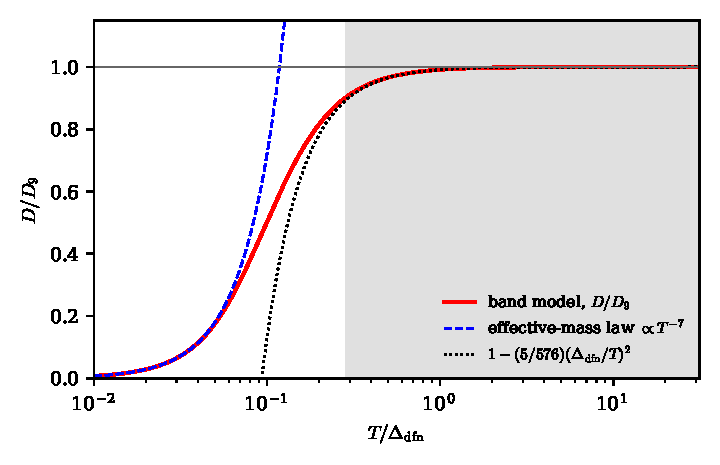
\includegraphics[width=0.75\linewidth]{figures/ch19/limit19_6a.pdf}
\captionof{figure}{Diffusion constant of a defecton in a simple cubic tight-binding band, \cref{eq:19.6-D}, divided by its $T^{-9}$ limit $D_9$, against the temperature in units of the band width. The ratio depends on $T/\Delta_{\mathrm{dfn}}$ alone, since the phonon rate $\varGamma_{k^2}$ of \cref{eq:19.6-q2} cancels. Red: the band model, crystal momentum diffusing at a constant rate with the detailed-balance drift. Blue dashed: the effective-mass law $D = 6T^2/\varGamma_{k^2} \propto T^{-7}$. Dotted: the leading correction $1 - \tfrac{5}{576}(\Delta_{\mathrm{dfn}}/T)^2$. Gray: within \SI{10}{\percent} of the $T^{-9}$ law, $T \ge 0.28\,\Delta_{\mathrm{dfn}}$. The upper edge $T \ll \theta_p$ lies outside the plot and depends on the crystal.}\label{fig:19-limit-defecton}
\par}
\smallskip
Below $0.28\,\Delta_{\mathrm{dfn}}$ the band is no longer uniformly populated and the law steepens toward $T^{-7}$; above $\theta_p$ the phonons are no longer long-wave and the Rayleigh law of the cross-section fails.
\end{limitbox}

The $T^{-9}$ law holds better than its derivation suggests. The ratio $D/D_9$ expands as $1 - (5/16)(A_{\mathrm{dfn}}/T)^2$, so the law is within \SI{10}{\percent} for $T \ge 0.28\,\Delta_{\mathrm{dfn}}$ and within \SI{1}{\percent} for $T \ge 0.93\,\Delta_{\mathrm{dfn}}$, although the condition stated with it is $T \gg \Delta_{\mathrm{dfn}}$. The relevant energy is the hopping amplitude, a sixth of the band width. At $T = 0.1\,\Delta_{\mathrm{dfn}}$ the local exponent is $-7.9$. A defecton moves faster the colder the crystal, until strain gradients localize it. In a real crystal the gradients from impurities, dislocations and the defect's own partner set $R_0$, and a band narrower than the elastic interaction at a few lattice spacings never carries the defect far.

\subsection{Crowdions}\label{sec:19.6-crowdion}

An extra atom in a close-packed row of a body-centered cubic metal spreads over many neighbors as a kink in the row, a crowdion. In tungsten, the metal of many transition-edge sensors, the self-interstitial takes this form along $\langle111\rangle$~\cite{fitzgerald2018structure}. The Frenkel--Kontorova chain of \cref{app:C.20} describes it: atoms of mass $M_\kappa$ at spacing $a_{\mathrm{ch}}$, springs $K_{\mathrm{ch}}$, and the potential $V_{\mathrm{s}}\sin^2(\pi z/a_{\mathrm{ch}})$ of the surrounding crystal, \cref{eq:C.20-FK}. For a slowly varying displacement the chain obeys the sine-Gordon equation, and its kink has the profile \cref{eq:C.20-kink} of width $d_{\mathrm{kink}} = a_{\mathrm{ch}}^2[K_{\mathrm{ch}}/2\pi^2V_{\mathrm{s}}]^{1/2}$~\cite[Eq.~(2)]{fitzgerald2018structure} and the rest energy $E_{\mathrm{kink}} = 4V_{\mathrm{s}}d_{\mathrm{kink}}/a_{\mathrm{ch}}$ of \cref{eq:C.20-Ekink}~\cite[Eq.~(3)]{fitzgerald2018structure}. The crowdion moves as a particle of mass
\begin{equation}
  M_{\mathrm{cr}} = \frac{2}{\pi^2}\,\frac{a_{\mathrm{ch}}}{d_{\mathrm{kink}}}\,M_\kappa ,
  \label{eq:19.6-Mcr}
\end{equation}
the kink mass \cref{eq:C.20-mass}~\cite{braun2004frenkel}, and the discrete row makes it cross the Peierls--Nabarro barrier $E_{\mathrm{PN}}$ of \cref{eq:C.20-EPN} to move by one spacing.

For tungsten, $V_{\mathrm{s}} \approx \SI{1}{eV}$ and $K_{\mathrm{ch}}a_{\mathrm{ch}}^2 = 50$ to \SI{100}{eV} are typical values~\cite{fitzgerald2018structure}. They give $d_{\mathrm{kink}} = 1.59$ to $2.25\,a_{\mathrm{ch}}$, $E_{\mathrm{kink}} = 6.4$ to \SI{9.0}{eV}, $M_{\mathrm{cr}} = 0.127$ to $0.090\,M_\kappa$ and a barrier of $1.2\times10^{-4}$ to $3.6\times10^{-7}\,\si{eV}$, with $a_{\mathrm{ch}} = \frac{\sqrt3}{2}\times\SI{3.165}{\angstrom} = \SI{2.741}{\angstrom}$. Atomistic calculations put the barrier near a meV instead~\cite{fitzgerald2018structure}, because the real substrate potential of tungsten is not a single sine. A particle of mass $M_{\mathrm{cr}}$ in the periodic potential $\tfrac12E_{\mathrm{PN}}[1 - \cos(2\pi z_0/a_{\mathrm{ch}})]$ has a ground band whose width follows from Mathieu's equation. The free-recoil energy $\pi^2/2M_{\mathrm{cr}}a_{\mathrm{ch}}^2$ is \SI{0.12}{meV} for the narrower kink, equal to its barrier within \SI{3}{\percent}, and \SI{0.17}{meV} for the wider one, and the band is 90 to \SI{166}{\micro eV}, 1.0 to \SI{1.9}{K}. With the atomistic barrier of \SI{1}{meV} and the same masses it narrows to 13 to \SI{34}{\micro eV}, 0.15 to \SI{0.39}{K}. Either way the band is wider than the temperature of a detector, so a crowdion is a candidate for coherent motion at millikelvin, a defecton of one dimension.

\begin{limitbox}[Crowdion profile and kink mass][lim:19.6b]
The published crowdion is the sine-Gordon kink \cref{eq:C.20-kink} with rest energy \cref{eq:C.20-Ekink}~\cite[Eqs.~(2), (3)]{fitzgerald2018structure}, of mass \cref{eq:19.6-Mcr} and barrier \cref{eq:C.20-EPN}.
\par\smallskip
{\centering
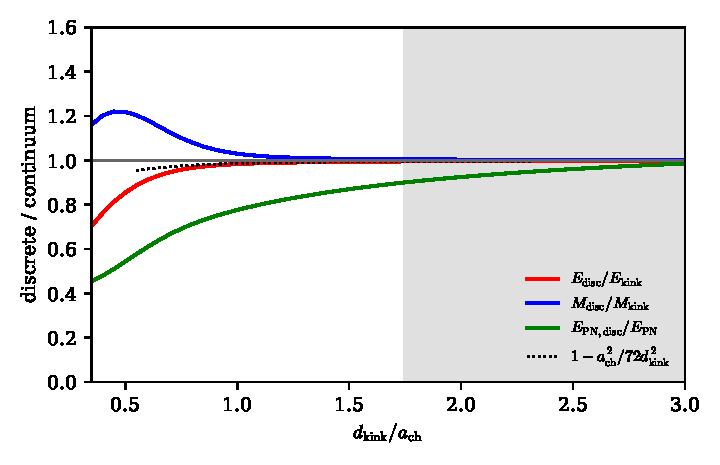
\includegraphics[width=0.75\linewidth]{figures/ch19/limit19_6b.pdf}
\captionof{figure}{Discrete Frenkel--Kontorova crowdion against the continuum kink, as ratios, against the kink width in units of the row spacing. The discrete chain of \cref{eq:C.20-FK} is relaxed numerically with the kink centered between two atoms (the minimum) and on an atom (the saddle). Red: rest energy, against $E_{\mathrm{kink}}$. Blue: translation mass $M_\kappa\sum_n(u_{n+1} - u_n)^2/a_{\mathrm{ch}}^2$, the lattice form of $M_\kappa\sum_n(\partial u_n/\partial z_0)^2$, against \cref{eq:19.6-Mcr}. Green: saddle minus minimum, against $E_{\mathrm{PN}}$ of \cref{eq:C.20-EPN}. Dotted: the leading correction to the energy, $1 - a_{\mathrm{ch}}^2/72d_{\mathrm{kink}}^2$. Gray: all three within \SI{10}{\percent}, $d_{\mathrm{kink}} \ge 1.74\,a_{\mathrm{ch}}$, set by the barrier.}\label{fig:19-limit-crowdion}
\par}
\smallskip
Well below one row spacing the kink is no longer a smooth profile: the barrier falls to half the continuum value near $0.4\,a_{\mathrm{ch}}$, and the mass and energy deviate by tens of percent.
\end{limitbox}

The energy and the mass of the kink hold far beyond the barrier. Replacing the spring energy $\frac12K_{\mathrm{ch}}\sum(u_{n+1} - u_n)^2$ by its continuum form drops the next term of $4\sin^2(ka_{\mathrm{ch}}/2) = k^2a_{\mathrm{ch}}^2 - k^4a_{\mathrm{ch}}^4/12$, which is $-(K_{\mathrm{ch}}a_{\mathrm{ch}}^3/24)\int\dd z\,u''^2$. On the kink, $\int\dd z\,u''^2 = 2a_{\mathrm{ch}}^2/3\pi^2d_{\mathrm{kink}}^3$, and to first order the energy changes by $-K_{\mathrm{ch}}a_{\mathrm{ch}}^5/36\pi^2d_{\mathrm{kink}}^3 = -E_{\mathrm{kink}}\,a_{\mathrm{ch}}^2/72d_{\mathrm{kink}}^2$, \SI{1.4}{\percent} at $d_{\mathrm{kink}} = a_{\mathrm{ch}}$. The discrete energy follows this law within $2\times10^{-4}$ above $1.5\,a_{\mathrm{ch}}$, and the mass exceeds \cref{eq:19.6-Mcr} by \SI{3}{\percent} at one spacing and by less beyond. The barrier is the weak point, \SI{22}{\percent} below \cref{eq:C.20-EPN} at $d_{\mathrm{kink}} = a_{\mathrm{ch}}$ and \SI{7.5}{\percent} below at $2\,a_{\mathrm{ch}}$, because it is exponentially small and the relaxation of the discrete chain changes it at the same order. For tungsten the model lies inside the shaded region for the stiffer chain and just below its edge for the softer one, so the mass is reliable and the barrier is not, as the atomistic meV already shows.

The conduction electrons, the phonons and the strain field of the parent vacancy decide whether the band survives in a real metal. Bulk tungsten is a normal metal above about \SI{15}{mK}, so its conduction electrons dress the hopping by a power of the ohmic coupling $\alpha_{\mathrm{ohm}}$ and, for $\alpha_{\mathrm{ohm}} < 1/2$, damp the coherent motion above a temperature of order $\Delta_{\mathrm{r}}/\pi\alpha_{\mathrm{ohm}}$, with $\Delta_{\mathrm{r}}$ the renormalized tunneling amplitude of \cref{sec:16.8-ohmic}. The phonons that distinguish neighboring positions multiply the hopping by $\ee^{-S_{\mathrm{pol}}(T)}$ of \cref{eq:E.22-Spol}, which has not been estimated for a crowdion. The strain field of the vacancy left behind confines the crowdion within $R_0$ of it: for an elastic interaction constant of about \SI{1}{eV}, an assumption, and a band of 13 to \SI{166}{\micro eV}, $R_0 = 12$ to 22 spacings. Inside $R_0$ the crowdion slides down the gradient toward its vacancy, and its recombination time is a drift time, peaked, not the $t^{-3/2}$ tail of a free random walk. The Peierls profile, the phonon coupling and the interaction with the parent vacancy remain to be computed with density-functional theory in a tungsten cell.

\subsection{The low-energy excess}\label{sec:19.6-lee}

Cryogenic detectors of many materials and designs record excess events whose spectra rise toward threshold, from tens of eV to a few keV~\cite{adari2022excess}. In the measurement of Anthony-Petersen and collaborators, two silicon crystals of $1\times1\times\SI{0.1}{cm^3}$, with identical sensors made on one wafer, were mounted in two ways: one glued to its copper holder with varnish, the other hung from aluminum wire bonds~\cite{anthonypetersen2024stress}. In energy absorbed by the sensor, the glued crystal shows a rate between 3 and \SI{38}{eV} more than two orders of magnitude above the suspended one. The rates in the 3--38 and 38--\SI{85}{eV} bins fall with time constants of 6 to 10 days after cooldown, while the rate above \SI{85}{eV}, from muons and radioactivity, stays constant. A single exponential does not describe the lowest bin of the glued crystal, with $\chi^2 = 4192$ for 68 degrees of freedom~\cite[Sect.~II\,B]{anthonypetersen2024stress}. In germanium detectors without a charge signal, the shape of the excess stays fixed while its rate falls slowly, the rate jumps after the detectors are warmed above \SI{10}{K}, and tests with adjustable stress on the crystal and different holders show no significant effect. One leading hypothesis there is the cracking of the epoxy that glues the thermistor to the crystal~\cite[Sect.~2.1.2]{adari2022excess}.

Energy conservation bounds what any defect source can supply, whatever the model. A source fed by particle events releases at most the energy those events stored, by \cref{eq:19.6-sumrule}: over any interval it releases the sum of $E_{\mathrm{st},k}(t_1) - E_{\mathrm{st},k}(t_2)$ over the events $k$ that seeded it. A source of elastic energy relaxing since cooldown releases at most the decrease of its relaxable elastic energy $U_{\mathrm{rel}}$. Point defects grown into the crystal or frozen in at cooldown release at most the decrease of their stored energy $E_{\mathrm{st},0}$, by the same sum rule. The energy recorded in excess events over $[t_1, t_2]$ obeys
\begin{multline}
  \int_{t_1}^{t_2}\dd t\int\dd E\;E\,\frac{\dd\mathcal{R}_{\mathrm{LEE}}}{\dd E\,\dd t}
  \le f_{\mathrm{ph}}\Bigl\{\bigl[U_{\mathrm{rel}}(t_1) - U_{\mathrm{rel}}(t_2)\bigr] + \bigl[E_{\mathrm{st},0}(t_1) - E_{\mathrm{st},0}(t_2)\bigr] \\
  + \sum_k\bigl[E_{\mathrm{st},k}(t_1) - E_{\mathrm{st},k}(t_2)\bigr]\Bigr\} ,
  \label{eq:19.6-leebound}
\end{multline}
with $f_{\mathrm{ph}} \le 1$ the largest collected fraction. The same bound holds for each event separately. Three consequences follow without any model: the event-seeded term is small, a single release must be large, and two crystals that differ in mounting differ in their elastic energy. First, electron recoils below \SI{0.14}{MeV} cannot displace atoms (\cref{sec:19.5-yield}), and a \SI{10}{eV} electron gives a silicon nucleus at most $4m_eE/M_\kappa = \SI{0.78}{meV}$. Nuclear recoils store at most \SI{5.5}{\percent} of their energy in silicon and \SI{6.4}{\percent} in germanium at \SI{95}{\percent} confidence (\cref{tab:19-bounds}). These bounds hold under the conditions of \cref{sec:19.5-yield}, and the silicon bound loosens to 0.081 at $\mathfrak{r}_{\mathrm{coll}} = 0.9$. Either way, the stored energy of the recoils a detector has seen is a small fraction of the energy it has already recorded from them. Second, at $f_{\mathrm{ph}} = 0.25$ an event of \SI{3}{eV} needs \SI{12}{eV} released at once, and one of \SI{38}{eV} needs \SI{152}{eV}, the energy of 22 close Frenkel pairs or of a pocket of about 1500 atoms. Third, two crystals cut from one wafer, with the same exposure to particles and the same grown-in defects, differ in mounting by $U_{\mathrm{rel}}$, provided that mounting changes neither $f_{\mathrm{ph}}$ nor the rates of stress-assisted defect reactions. The factor of more than a hundred between them then reflects elastic energy, not defects from radiation or growth. The excess events are therefore collective releases of energy stored at cooldown, and the open question is how they happen.

A collective-release model rests on three hypotheses: a reservoir of relaxable elastic energy, relaxation rates spread uniformly in $\ln\varGamma$, and a fixed law for the energies of single events. The reservoir $U_{\mathrm{rel}}$ is stored at cooldown in the crystal, the glue and the interfaces of the holder, and it relaxes by local events, thermally activated or tunneling, with rates between $\varGamma_{\min}$ and $\varGamma_{\max}$, spread as the barriers of a glass are (\cref{sec:16.8-heat}). We write the law of single-event energies as $p_{\mathrm{LEE}}(E)$. The second hypothesis fixes the time law by the argument of \cref{eq:16.8-heat}: the fraction relaxing per unit time is $1/[t\ln(\varGamma_{\max}/\varGamma_{\min})]$ for $\varGamma_{\max}^{-1} \ll t \ll \varGamma_{\min}^{-1}$, so each factor $\ee$ in time releases $U_{\mathrm{rel}}/\ln(\varGamma_{\max}/\varGamma_{\min})$. A fastest rate of order one per day bends the $1/t$ law at early times into the sum of exponentials that the data prefer. With $\langle E\rangle$ the mean of $p_{\mathrm{LEE}}$, the three together give
\begin{equation}
  \frac{\dd\mathcal{R}_{\mathrm{LEE}}}{\dd E\,\dd t} = \frac{f_{\mathrm{ph}}\,U_{\mathrm{rel}}}{\ln(\varGamma_{\max}/\varGamma_{\min})\,\langle E\rangle}\,\frac{p_{\mathrm{LEE}}(E)}{t} .
  \label{eq:19.6-lee}
\end{equation}
The size law comes from triggering. If the phonons of one release trigger on average $b_{\mathrm{br}}$ further releases, as in \cref{sec:16.8-open}, and the number triggered is Poisson, the total number $N_{\mathrm{casc}}$ in one cascade follows the Borel distribution
\begin{equation}
  P(N_{\mathrm{casc}}) = \frac{\ee^{-b_{\mathrm{br}}N_{\mathrm{casc}}}\,(b_{\mathrm{br}}N_{\mathrm{casc}})^{N_{\mathrm{casc}} - 1}}{N_{\mathrm{casc}}!} ,
  \label{eq:19.6-borel}
\end{equation}
with mean $1/(1 - b_{\mathrm{br}})$. By Stirling's formula it falls as $N_{\mathrm{casc}}^{-3/2}\ee^{-N_{\mathrm{casc}}(b_{\mathrm{br}} - 1 - \ln b_{\mathrm{br}})}$, a power law $N_{\mathrm{casc}}^{-3/2}$ cut off at $N_{\mathrm{casc}} \sim 2/(1 - b_{\mathrm{br}})^2$ near the critical value $b_{\mathrm{br}} = 1$. Such a cascade of elementary releases produces a spectrum that rises toward threshold as a power with an exponential cutoff.

The model predicts how the excess scales, not its rate. The rate is proportional to $U_{\mathrm{rel}}$, which for a layer under thermal-mismatch stress $\sigma_{\mathrm{str}}$ is of order $\sigma_{\mathrm{str}}^2\Vol/Y_{\mathrm{mod}}$ of the relaxing component, with $Y_{\mathrm{mod}}$ its Young's modulus. A glue layer on a clamped crystal dominates, and the factor of a hundred between glued and suspended crystals is a ratio of $U_{\mathrm{rel}}$ that a thermo-elastic calculation can test. The clock restarts when the relaxing component is warmed above the temperature at which it creeps, as in the jumps after warming above \SI{10}{K}. A stress applied to the bulk of a crystal that does not creep adds little $U_{\mathrm{rel}}$, which agrees with the null results under adjustable stress if the source lies in the glue of the thermistor. The shape of the spectrum and its time dependence factorize, so the shape does not change as the rate falls, as observed in germanium. A rate needs two inputs that do not exist: $U_{\mathrm{rel}}$ with its spread of rates $[\varGamma_{\min}, \varGamma_{\max}]$ for a given holder and glue, and the branching ratio $b_{\mathrm{br}}$, which fixes the size law. The first comes from a finite-element calculation of the cooldown stress with measured elastic and expansion data, with the relaxable fraction from low-temperature mechanical data of the glue. The second comes from the catalogue of release paths and the transport of the phonon pulse of one release. A fit of \cref{eq:19.6-lee} with these inputs to a glued and an unglued crystal would then have no free parameter.

\subsection{Open problems}\label{sec:19.6-open}

The release of close Frenkel pairs in silicon and germanium, and of split interstitials in aluminum, at millikelvin (\cref{sec:19.6-kinetics}) needs one calculation per path: the tunneling exponent along the computed minimum-energy path and $E_{\mathrm{reorg}}/\varepsilon^{\mathrm{hop}}$, both to about \SI{5}{\percent}.

In ionic crystals the electronic route to stored energy is prompt. A self-trapped exciton can turn into a close pair of an F center and an interstitial within picoseconds. Part of the energy of an electron recoil is then stored before the partition time, and the electron-recoil calibration of such crystals has a heat deficit too. Per unit deposit the stored energy is the number of excitons per unit energy times the conversion probability, the survival probability of the close pair and its configurational energy. The conversion probability at millikelvin and the survival of the close pair against tunneling recombination are not known.

Carriers of later events can drive defect reactions without heat. A capture or recombination at a defect puts energy into its local modes, and if the reaction coordinate is coupled linearly with Huang--Rhys factor $S_{\mathrm{HR,rxn}}$ and energy $\omega_{\mathrm{rxn}}$, the number of quanta it receives at $T = 0$ is Poisson (\cref{eq:5.6-poisson}). The probability that one capture drives the reaction over a barrier $V_{\mathrm{b}}$ is the tail
\begin{equation}
  p_{\mathrm{rxn}} = \sum_{n \ge V_{\mathrm{b}}/\omega_{\mathrm{rxn}}}\ee^{-S_{\mathrm{HR,rxn}}}\,\frac{S_{\mathrm{HR,rxn}}^n}{n!} ,
  \label{eq:19.6-prxn}
\end{equation}
and the stimulated rate is the capture rate times $p_{\mathrm{rxn}}$. It enters \cref{eq:19.6-master} as a time-dependent rate, so \cref{eq:19.6-sumrule} still holds. The Huang--Rhys factor, the mode energy and the barrier of real defects, with the change of charge state, are not computed.

\subsection{Uncertainty budget of the nuclear-recoil response}\label{sec:19.6-budget}

\Cref{tab:19-nuisances} collects the truncations and inputs of the chapter with their sizes.
\begin{table}[tbp]
  \caption{Uncertainty budget of the low-energy nuclear-recoil response. Classes and bases as in \cref{tab:10-nuisances}; ``delayed'' moves energy in time without changing the prompt yield.}
  \label{tab:19-nuisances}
  \centering\scriptsize\setlength{\tabcolsep}{3pt}
  \begin{tabular}{@{}>{\raggedright\arraybackslash}p{0.26\linewidth}>{\raggedright\arraybackslash}p{0.12\linewidth}>{\raggedright\arraybackslash}p{0.35\linewidth}>{\raggedright\arraybackslash}p{0.09\linewidth}>{\raggedright\arraybackslash}p{0.10\linewidth}@{}}
    \toprule
    Truncation or input & Type & Size & Basis & Section \\
    \midrule
    Classical propagation of the kicked Wigner ensemble & tilt & misses the third cumulant (share $\propto x_R^{-1/2}$) and quantum effects after the kick & computed & \cref{sec:19.1} \\
    Regime boundaries of the recoil dynamics & threshold & silicon 0.41, \SI{0.54}{eV}; 12.5--\SI{36}{eV}; 0.87--\SI{4.6}{keV}, at a criterion of 0.1 & est. & \cref{sec:19.1} \\
    Machine-learned surface along the recoil path & threshold; normali\-zation & thresholds to the \SI{0.7}{eV} step width; a few tenths of an eV per defect & input spread & \cref{sec:19.1} \\
    Charge below the binary threshold & normali\-zation; threshold & silicon yield 0.10 at \SI{100}{eV}; close-collision kernel not computed & unsized & \cref{sec:19.2} \\
    Migdal part of a measured yield & normali\-zation & 2.3--$4.4\times10^{-4}$ in $Y_q$, at most \SI{0.4}{\percent} at \SI{100}{eV} & computed & \cref{sec:19.2} \\
    Lindhard quenching below a few keV & normali\-zation & data 8--\SI{38}{\percent} below the formula at 0.1--\SI{3.9}{keV}; soft-collision continuation $+$\SI{13}{\percent} at \SI{1}{keV} & input spread; model & \cref{sec:19.3} \\
    Prefactor of the displacement count & normali\-zation & 0.70 (screened) against 0.8 (formula) and 1 (hard spheres) & computed & \cref{sec:19.4} \\
    Stored share of a nuclear recoil & normali\-zation (heat) & at most 0.055 (Si; 0.049 with the measured pair energy) and 0.064 (Ge), \SI{95}{\percent} C.L., under (a)--(e); Si 0.081 at $\mathfrak{r}_{\mathrm{coll}} = 0.9$ & input spread & \cref{sec:19.5} \\
    Gap energy unreturned in the read window & normali\-zation (heat) & $Y_{\mathrm{ph}}(0) = 1.407$ at \SI{100}{eV} with none returned; \SI{1}{\percent} needs at most 3.5--\SI{4.1}{\percent} unreturned & computed & \cref{sec:19.5} \\
    Collection ratio of Luke phonons & normali\-zation & 1.128 alone reproduces the silicon datum; transport estimate 0.81--1.02 & computed & \cref{sec:19.5} \\
    Pair energy adopted by the reconstruction & normali\-zation & $-0.0064$ in $Y_{\mathrm{ph}}$ at \SI{4}{V}, growing with bias & computed & \cref{sec:19.5} \\
    Collection offset from recombination phonons & normali\-zation & $\rho_g - 1 = 0.21$ gives the silicon deficit beyond the pair-energy offset & est. & \cref{sec:19.5} \\
    Collection ratio constant between two biases & normali\-zation & residual $(\dd\mathfrak{r}_{\mathrm{coll}}/\dd V_{\mathrm{bias}})\Delta V_{\mathrm{bias}}$ & unsized & \cref{sec:19.5} \\
    Zero-point change of the defect basins & normali\-zation (heat) & below \SI{0.1}{eV} per defect; widens the bounds by about $10^{-3}$ & est. & \cref{sec:19.5} \\
    Release of close pairs at millikelvin & delayed & frozen if weakly coupled; else needs an exponent 14 (Si) or \SI{6}{\percent} (Al) below the two-parabola value & est. & \cref{sec:19.6} \\
    Single releases in a phonon readout & new support & close pair 1.70--\SI{1.88}{eV} at a collected fraction of 0.25 & model & \cref{sec:19.6} \\
    Defecton and crowdion transport & delayed & $T^{-9}$ law within \SI{10}{\percent} for $T \ge 0.28\,\Delta_{\mathrm{dfn}}$; crowdion barrier $-$\SI{22}{\percent} at $d_{\mathrm{kink}} = a_{\mathrm{ch}}$ & model & \cref{sec:19.6} \\
    Rate of the low-energy excess & new support & relaxable elastic energy and branching ratio not computed & unsized & \cref{sec:19.6} \\
    \bottomrule
  \end{tabular}
\end{table}
